\section{Readout system}
\label{sec:readout}
A precise and stable electronic readout system is needed to achieve the required precision. In previous versions of the calibration system, each sensor was connected to a different and independent electronic circuit and thus, fed by a different current and read by a different ADC channel. It was soon realized that the measured temperature difference between any two pairs of sensors was heavily affected by the electronic offset between channels. This offset was not constant, and showed dependence on ambient temperature and humidity, which affected both the current source and the ADC, generating variations of tens of mK for the measurement of a single calibration constant between sensors. A variant of an existing mass PT100 temperature readout system developed at CERN for one of the LHC experiments \cite{bib:multiplexing_board} was adapted to solve this problem. The system consists of an electronic circuit that includes:

\begin{itemize}
\item A precise and accurate 1 mA current source for the excitation of the temperature sensors. Based on an application of the Texas Instruments precise voltage reference REF102CU with a possibility to adjust ±10nA with Keithley 2001 multimeter \cite{xavier,keithley}.%This source is adjusted to the 10 nA level with a Keithley 2001 multimeter \cite{keithley}. 
\item A multiplexing circuit based on the Analog Devices ADG1407BRUZ multiplexer with ultralow internal resistance in an 8-channel differential configuration. The readout circuit contains three multiplexers, providing a readout capacity of 24 channels. The multiplexing circuit and the current sourced are realised in a single card (see Fig.~\ref{fig:readout}). 
\item A readout system based on National Instruments Compact RIO-FPGA device \cite{compactrio} equipped with a NI-9238 analogue input module that provide 24 bits of resolution over 1 Volt range \cite{ni9238}. By programming the Van Dusen equation the readout calculates the temperature in Kelvin units. The Compact RIO also drives the control bits of the multiplexers
\end{itemize}

\begin{figure}[htbp]
\centering
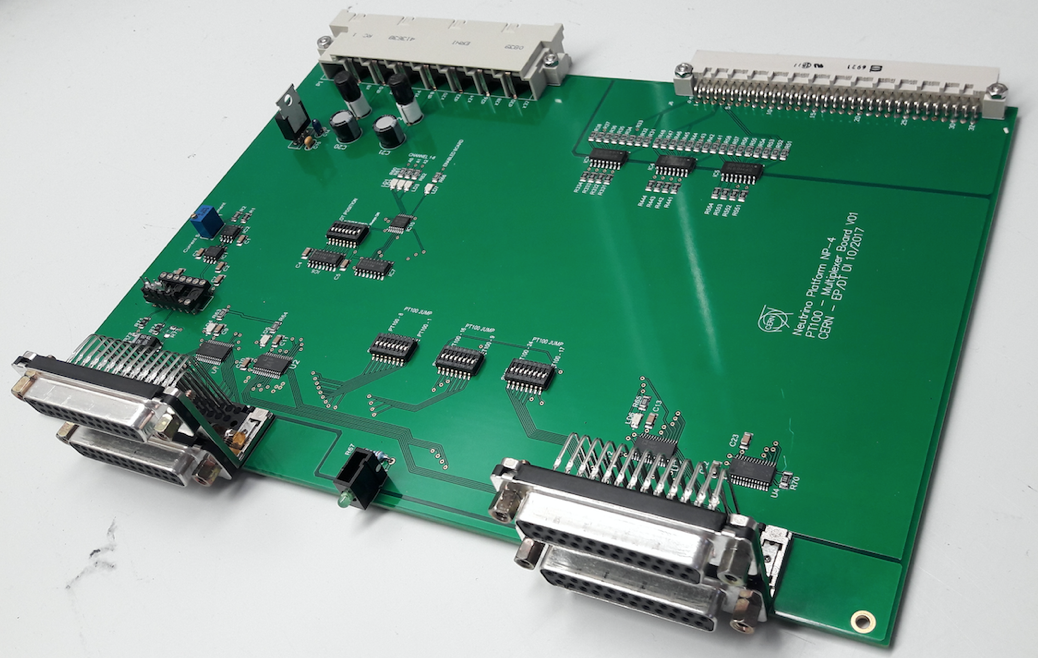
\includegraphics[width=0.6\textwidth]{images/figure_2.png}
\caption{Current source and multiplexing card with 24 channels. 
\label{fig:readout}}
\end{figure}

\noindent
One of the features of the readout circuit is the serialization of the current source excitation for all the sensors connected to the same board. The same 1 mA current is delivered to all sensors connected to the same board. Multiplexing the signal of the sensors such that they can be readout by the same ADC channel minimises the residual offset due to the electronics. This system was used during the calibration campaigns presented in this article and also for the temperature measurements during ProtoDUNE-SP operation. 

The readout was not considered a potential source of bias during the calibration campaign prior to the installation in ProtoDUNE-SP (see Sec.~\ref{sec:old_calib}) and it was not studied in detail at that time. However, aiming to improve the calibration results after ProtoDUNE-SP operation, a more thoughtful study of the readout was performed before the calibration campaigns presented in Sec.~\ref{sec:new_calib}. In particular, the twelve channels (7-18) used for sensor calibration were investigated. It was found that, despite the multiplexing system, a small residual offset between channels still exists. Figure \ref{fig:readout_calib} shows the offsets of channels 8-18 with respect to channel 7, computed using twelve 20 ohms low Temperature Coefficient of Resistance (TCR)\footnote{The temperature coefficient of resistance is defined as the change in resistance per unit resistance per degree rise in temperature. Typically ±5ppm/°C.} precision resistors, with an equivalent temperature of 76 K. Two of those, High Precision 1 (HP1) and High Precision 2 (HP2), are selected as the measurement samples and connected to the reference channel (7) and the channel being calibrated (from 8-18), while leaving all other channels connected to other secondary resistors to let the current flow through the system. The readout offset between channel 7 and channel X, $\Delta T_{7-X}^{readout}$, is then computed using the results of two consecutive measurements:

\begin{enumerate}%[label=(\Alph*)]
    \item HP1 in channel 7 and HP2 in the channel X being calibrated. The offset between the measured temperatures is 

    \begin{equation}
        \Delta T_{7-X}^A = T_{X}^{HP2}-T_{7}^{HP1}+\Delta T_{7-X}^{readout} \, .
    \end{equation}  
    
    \item HP2 channel 7 and HP1 in the channel X being calibrated. The offset between the measured temperatures is
\end{enumerate}

    \begin{equation}
        \Delta T_{X-7}^B = T_{X}^{HP1}-T_{7}^{HP2}+\Delta T_{7-X}^{readout} \, .
    \end{equation}  

\noindent 
Because of the very low TCR of the resistors, it can be assumed that the resistances are constants in those two measurements ( $T_{7}^{HP1}=T_{X}^{HP1}$ and $T_{7}^{HP2}=T_{X}^{HP2}$). Thus, the offset between channels 7 and X can be computed as the average between those two measurements: 

\begin{equation}
    \Delta T_{7-X}^{readout} = \frac{\Delta T^{A}_{7-X} + \Delta T^{B}_{X-7}}{2} \, .
\end{equation}

The results in Fig.~\ref{fig:readout_calib}, show an offset of up to 2.5 mK when comparing directly with channel 7, while the offset between any other two channels is below 1 mK, indicating that there is something special about the first channel being readout. Error bars in that figure correspond to the RMS of four independent measurements (repeatability) of the same offset (see Fig.~\ref{fig:readout_calib}). As it can be observed the error is below 0.5 mK, what probes the great repeatability of the readout. These offsets are more likely due to parasitic resistances in the different lines that are multiplexed. This finding allowed a correction to the measurements taken during the subsequent calibration campaigns, improving the obtained precision. 

\begin{figure}[htbp]
\centering
{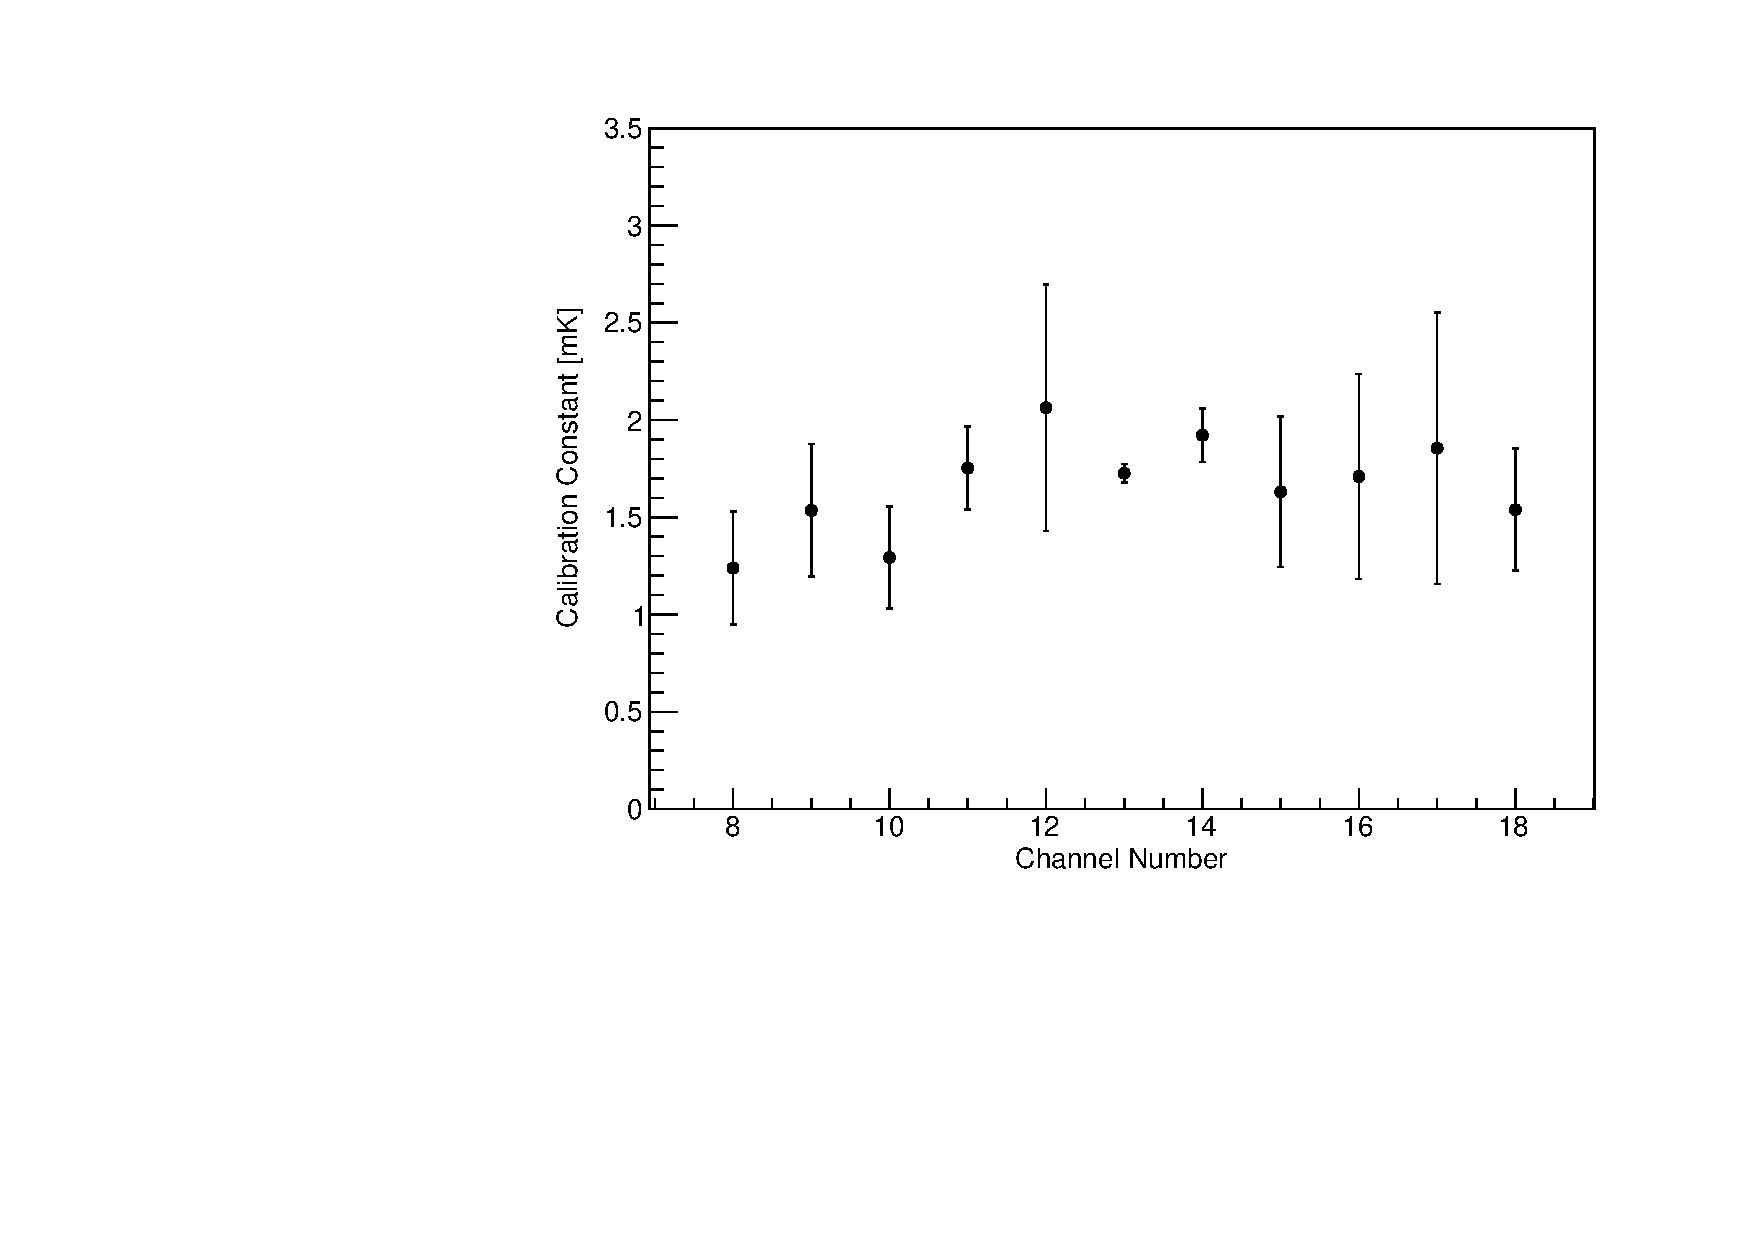
\includegraphics[width=0.65\textwidth]{images/figure_3.pdf}}
\caption{Offset between readout channels 8-18 and channel 7, used as reference. Points correspond to the mean of the 4 independent measurements and the error bars are their RMS.}
\label{fig:readout_calib}
\end{figure}